%% Le lingue utilizzate, che verranno passate come opzioni al pacchetto babel. Come sempre, l'ultima indicata sar� quella primaria.
%% Se si utilizzano una o pi� lingue diverse da "italian" o "english", leggere le istruzioni in fondo.
\def\thudbabelopt{italian,english}
%% Valori ammessi per target: bach (tesi triennale), mst (tesi magistrale), phd (tesi di dottorato).
%% Valori ammessi per aauheader: '' (vuoto -> nessun header Alpen Adria Univeristat), aics (Department of Artificial Intelligence and Cybersecurity), informatics (Department of Informatics Systems). Il nome del dipartimento � allineato con la versione inglese del logo UniUD.
\documentclass[target=mst,aauheader=]{thud}

%% --- Informazioni sulla tesi ---
%% Per tutti i tipi di tesi
% Scommentare quello di interesse, o mettete quello che vi pare
\course{Informatica}
%\course{Internet of Things, Big Data e Web}
%\course{Matematica}
%\course{Comunicazione Multimediale e Tecnologie dell'Informazione}
\title{A DLT-based application for certifying journalistic material}
\author{Andrea Vendrame}
%% Campi obbligatori: \title, \author e \course.
%% Altri campi disponibili: \reviewer, \tutor, \chair, \date (anno accademico, calcolato in automatico), \rights
%% Con \supervisor, \cosupervisor, \reviewer e \tutor si possono indicare pi� nomi separati da \and.

%% --- Pacchetti consigliati ---
%% pdfx: per generare il PDF/A per l'archiviazione. Necessario solo per la versione finale
\usepackage[a-1b]{pdfx}
%% hyperref: Regola le impostazioni della creazione del PDF... pi� tante altre cose. Ricordarsi di usare l'opzione pdfa.
\usepackage[pdfa]{hyperref}
%% tocbibind: Inserisce nell'indice anche la lista delle figure, la bibliografia, ecc.
\usepackage{graphicx}

%% --- Stili di pagina disponibili (comando \pagestyle) ---
%% sfbig (predefinito): Apertura delle parti e dei capitoli col numero grande; titoli delle parti e dei capitoli e intestazioni di pagina in sans serif.
%% big: Come "sfbig", solo serif.
%% plain: Apertura delle parti e dei capitoli tradizionali di LaTeX; intestazioni di pagina come "big".

\begin{document}
\maketitle

%% Dedica (opzionale)
\begin{dedication}
	Al mio cane,\par per avermi ascoltato mentre ripassavo le lezioni.
\end{dedication}

%% Ringraziamenti (opzionali)
\acknowledgements
Sed vel lorem a arcu faucibus aliquet eu semper tortor. Aliquam dolor lacus, semper vitae ligula sed, blandit iaculis leo. Nam pharetra lobortis leo nec auctor. Pellentesque habitant morbi tristique senectus et netus et malesuada fames ac turpis egestas. Fusce ac risus pulvinar, congue eros non, interdum metus. Mauris tincidunt neque et aliquam imperdiet. Aenean ac tellus id nibh pellentesque pulvinar ut eu lacus. Proin tempor facilisis tortor, et hendrerit purus commodo laoreet. Quisque sed augue id ligula consectetur adipiscing. Vestibulum libero metus, lacinia ac vestibulum eu, varius non arcu. Nam et gravida velit.

%% Sommario (opzionale)
\abstract
The Truthster project is a decentralized application (dApp) that aims to provide a secure and reliable platform for journalists to share their interviews with their interviewees. The project is built on top of the Alastria blockchain network, which is a consortium blockchain network designed for the Spanish market.

One of the key features of Truthster is its ability to provide a high level of security and privacy to its users. The system uses advanced cryptographic techniques to ensure that files stored on the blockchain are tamper-proof and cannot be altered or deleted. Additionally, Truthster allows journalists to provide information about their identity, so that users can be sure that the files they are accessing are coming from a verified source.
The Alastria blockchain network is also designed to be highly scalable and efficient, in this way it can handle a large number of transactions per second, which is essential for a system that needs to process large amounts of data.

Another important aspect of the Truthster project is its user-friendly interface. The system is accessible through a web-based interface (client), which allows users to access their data from any device with an internet connection. Additionally, Truthster is designed to be intuitive and easy to navigate, making it accessible to users of all skill levels.

The Truthster project also aims to empower journalists by allowing them to share their work with a wider audience, while also ensuring that their interviewees can access the information with complete confidence. By providing a secure and reliable platform for sharing interviews, Truthster aims to promote transparency and trust in the media industry, which is a very difficult task nowadays.

In conclusion, the Truthster project is an innovative and valuable tool for journalism. It addresses the need for secure and reliable platforms for sharing interviews and provides a user-friendly experience. By leveraging the power of blockchain technology, the Truthster project aims to promote transparency and trust in the media industry, and empower journalists to share their work with a wider audience.

%% Indice
\tableofcontents

%% Lista delle tabelle (se presenti)
%\listoftables

%% Lista delle figure (se presenti)
%\listoffigures

%% Corpo principale del documento
\mainmatter

%% Parte
%% La suddivisione in parti � opzionale; solitamente sono sufficienti i capitoli.
%\part{Parte}

%% Capitolo
\chapter{Introduction}

The Truthster project aims at integrating an easy-to-use mobile application for certifying video interviews with a blockchain platform, thus generating proof of validity of media contents based on an innovative synergy between human trust (embodied by the interviewer) and trust- less systems (Alastria). Truthster will add to media creators an option to verify interviews, using a simple workflow combined with blockchain storage for proof of validity.\\

This project is a comprehensive solution that combines traditional technologies such as databases and REST architecture with new technologies like Docker and blockchain. The goal of the Truthster project is to create a mobile app that makes it easy for journalists and media creators to certify video interviews, providing proof of validity for media contents.\\

The mobile app is designed for the interviewer, who can use it to record audio or video interviews. Once the interview is recorded, the interviewer can open the mobile app, log in, enter all the related interview information, and choose the interview file to upload. The app then calculates a hash of the document (generated based on the information provided by the interviewer) and uploads it, along with interview metadata and GPS position, to a cloud-based server. In the background, the entire document and interview file are uploaded.\\

Once the interview is uploaded, the app sends a link to the interviewee via SMS or email, or generates a QR code with a link. The interviewee can then open the link (or scan the QR code), and a GDPR-compliant contract will be displayed for review and agreement.\\
After the contract is agreed upon, the GPS position of the interviewee is sent to the server, and the hash and metadata of the interview, along with the interviewee's agreement, are stored in a permissioned blockchain for later uses.\\

The blockchain used in the Truthster project is Alastria, an open-source and permissioned blockchain. This type of blockchain is a hybrid between a public blockchain (such as Ethereum or Moonriver) and a completely private blockchain (such as a local blockchain created with Ganache).\\
This allows for greater security and privacy, as only authorized individuals (such as registered journalists) have the right to write to the blockchain.\\

In addition to the blockchain, all media files and information are stored in a separate database, specifically a MongoDB instance. MongoDB is a document database that is highly available and scalable, making it well-suited for internet applications like ours. Its flexible schema approach is popular among development teams that use agile methodologies.\\

The Truthster project also includes a Node.js server that notifies the interviewer when the process is complete. A history of all interviews is also available to the interviewer through the mobile app, providing a convenient way to keep track of all interviews, explore past informations and handle other additional settings.\\

The backend server and web app are designed to be ready for the cloud, making it easy for media creators to access the Truthster system from anywhere. To further automate the development and operations process, the back-office module is implemented using Docker containers, allowing for easy deployment and scaling of the system.\\

Overall, the Truthster project is a unique and innovative solution that combines the trust of human interactions with the reliability and security of blockchain technology, providing a way for media creators to easily verify and certify video interviews. By using blockchain technology, the Truthster project ensures that the proof of validity of media contents is tamper-proof, providing a new level of trust for audiences.

%% Sezione
\section{Titolo della Sezione}

%% Sottosezione
\subsection{Sottosezione}





\chapter{State of the art}

The field of journalism and access to content is rapidly evolving, with new technologies and platforms emerging all the time. There is an increasing need for accurate, reliable, and verifiable information, as well as for tools that can help journalists to gather, produce, and distribute that information. At the same time, there is growing concern about the spread of misinformation and fake news, which makes it even more important to have tools that can help to verify the accuracy and authenticity of information. In response to these challenges, many new technologies and platforms have emerged that aim to improve the state of the art in journalism and content access, including tools for data journalism, fact-checking, and digital verification.\par
Some example of these categories include:

\begin{itemize} 

    \item \textbf{Factmata}\cite{factmata}: is a platform that uses AI and machine learning to provide digital verification and fact-checking services for news and other forms of content. It aims to combat misinformation and promote accuracy and credibility in journalism.
    \item \textbf{NewsWhip}\cite{NewsWhip}: Spike: is a tool designed for journalists, media organizations, and content creators to track and analyze the spread of news and content on social media. It provides real-time insights into what stories are resonating, who is driving engagement, and how audiences are interacting with different types of content.
    \item \textbf{Veracity.ai}\cite{veracity.ai/}: is a technology company that provides machine learning-powered solutions for verification and fact-checking in journalism and other industries. It offers a suite of tools that automate the process of verifying the authenticity of digital content and evaluating the credibility of sources. These tools use advanced algorithms to analyze large datasets and identify patterns and anomalies that can indicate the presence of false or misleading information. Veracity.ai aims to help organizations improve the accuracy and trustworthiness of their content, and enhance the efficiency and scalability of their fact-checking processes.
    \item \textbf{Factcheck.org}\cite{Factcheck}: is a non-partisan, non-profit organization dedicated to promoting accuracy in public discourse. It fact-checks statements from political figures, advocacy groups, and others and provides evidence-based analysis to help people better understand the issues and inform their decisions.
    \item \textbf{Media Bias/Fact Check}\cite{mediabiasfactcheck}: is a website that aims to assess the bias and accuracy of news sources. It provides information about the political bias of various news sources as well as evaluating the accuracy of specific claims made by these sources.
    \item \textbf{Google News Lab Verification Toolkit}\cite{googleVerificationToolkit}: is a set of resources and guidelines for journalists to help verify information and fight against misinformation. It includes a range of tools such as reverse image search, video verification, and fact-checking databases.

\end{itemize}

As we can notice many tools for data journalism, fact-checking, and digital verification are incorporating machine learning and AI models in their operations. The use of these technologies allows for more efficient and accurate processing of large amounts of data, as well as the ability to identify patterns, recognize misinformation, and provide verifiable insights. Machine learning and AI can also assist in automating certain fact-checking tasks and in detecting fake news and other forms of misinformation. With these advancements, journalists and fact-checkers are equipped with more powerful tools to ensure the accuracy and credibility of their work, and to provide the public with reliable and trustworthy information.\\

On the other side we have the users, the ones that access the contents provided by the journalism sphere. To ensure them authenticity and validity of digital contents there are several tools available today that can help with this need, particularly for video interviews.\\
Some of these include:

\begin{itemize}

    \item \textbf{Digital Signature}: is a way of verifying the authenticity and integrity of digital content. They work by using encryption to create a unique signature that is attached to the content. This signature can then be verified by anyone who receives the content to confirm that it has not been altered or tampered with during transmission. Some pros of digital signatures include increased security and trust in digital transactions, as well as ease of use and cost-effectiveness compared to traditional methods of authentication like hand-written signatures. On the other hand the cons of digital signatures include the need for a secure and trusted third-party certification authority to issue and manage the signatures, as well as potential vulnerability to hacking or technical failures. Additionally, there may be difficulties in ensuring the authenticity of the signer, as digital signatures do not necessarily prove the identity of the signer (something that in Truthster project is very important) in the same way that a hand-written signature does.
    \item \textbf{Hash-based Evidence Preservation (HBEP)}: is a method of preserving digital evidence using a cryptographic hash of the original content. HBEP aims to provide an immutable and tamper-proof record of digital content. The advantage of HBEP is that it provides a high level of security and immutability of digital content, as the hash of the content cannot be altered without changing the original content. However, one of the disadvantages of HBEP is that it requires the availability of the original content to verify the authenticity of the hash, making it difficult to use in some cases. Additionally, HBEP also requires a secure method of preserving the original content, as well as a secure method of distributing the hash of the content to ensure its authenticity.
    \item \textbf{Timestamping}: is a technique that allows you to associate a date and time with a piece of data or information. This technique is useful in various applications, including digital signatures, document management, and digital evidence preservation. Timestamping can provide an immutable record of when a particular piece of information was created, transmitted, or modified, making it an important tool for maintaining the integrity and authenticity of digital information. However, like any technology, timestamping also has some disadvantages. One of the biggest concerns with timestamping is that it relies on centralized authorities, such as trusted time servers, to provide the time stamp. This means that the accuracy of the time stamp is dependent on the accuracy and reliability of these centralized authorities, which can be vulnerable to tampering, malfeasance, or failures. Additionally, timestamping can also be resource-intensive, requiring significant computational resources and bandwidth to perform the time stamping process.
    \item \textbf{Blockchain}: is a decentralized, distributed ledger system that uses cryptography to secure its transactions and data. The most well-known application of blockchain is the cryptocurrency, Bitcoin (BTC is the token name). However, blockchain has potential applications in various industries such as finance, supply chain management, voting systems and also journalism. One of the major advantages of this technology is its high level of security, indeed it is nearly impossible to alter or manipulate the data once it is recorded on the ledger. Additionally, blockchain eliminates the need for intermediaries and increases transparency, as in general all participants in the network have access to the same information.\\However, there are also some cons associated with blockchain. For example, it is still a relatively new technology, and its scalability is limited. Additionally, the energy consumption associated with blockchain mining can be significant, and the cost of mining equipment and electricity can be high. Additionally, due to the decentralized nature of blockchain, there is no central authority to resolve disputes or correct errors, which can lead to confusion and issues.

\end{itemize}

All of these tools can be useful in ensuring the authenticity and validity of digital content, but they all have their own limitations.\\
Digital Signatures, HBEP and timestamping are methods that can ensure the authenticity of the content, but they don't provide a way to authenticate the identity of the interviewer and interviewee or to manage the consent of the interviewee. Blockchain-based platforms can solve this problem by allowing for the recording of the identities and consent of the parties involved, but they may have scalability issues.\\

In summary, Truthster aims to combine all of these tools in an easy-to-use, video-interview-focused, open and interoperable certification option for digital media.


\chapter{Blockchain}

The blockchain is a decentralized, digital ledger that records transactions across a network of computers in a secure, transparent, and tamper-proof way. Transactions are grouped into blocks, which are then linked and secured using cryptography. The result is a secure, tamper-proof, and transparent ledger that can be used to store and manage digital assets, such as cryptocurrencies, digital contracts (usually called smart contracts), and other types of data. Because the ledger is decentralized, it eliminates the need for intermediaries, such as banks or other financial institutions, to verify transactions, thus increasing efficiency and reducing costs. Additionally, the transparency of the ledger ensures that all parties have access to the same information, promoting trust and security. The blockchain is an innovative technology that has the potential to transform various industries, including finance, supply chain management, and identity management.

\indent In this chapter, we will delve into the intricacies of the blockchain technology by examining its various components and how it works. We will also provide implementation examples of this technology to help you understand its practical applications. In addition, we will discuss some of the advantages and disadvantages of the technology with past real use cases to give you a well-rounded understanding of the subject. Through this chapter, our aim is to provide a comprehensive overview of the blockchain and its components so that you can gain a deeper understanding of the technology and its potential impact on various industries.

\section{Blockchain components}

At a high level we can see the blockchain as an aggretation of the following components that exist and work together to provide a service to the end user:

\begin{enumerate}

    \item Blocks: a blockchain is a chain of blocks, where each block contains a collection of data and a unique identifier called "hash".
    \item Nodes: a node is a computer connected to the blockchain network and participating in the network's consensus process.
    \item Network: a network is a group of interconnected devices that can communicate and exchange information with each other.
    \item Transaction: a transaction is a transfer of value between users in a blockchain network.
    \item Cryptographic Hash function: A hash function is a mathematical algorithm that takes in data and outputs a fixed-size string of characters, called a "hash." The hash serves as a unique identifier for each block in the blockchain.
    \item Consensus algorithm: A consensus algorithm is a mechanism that ensures that all nodes on the network agree on the current state of the blockchain.
    \item Smart Contracts: a smart contract is a self-executing agreement with the terms of the agreement directly written into lines of code.
    \item Public/private key cryptography: Public/private key cryptography is used to secure the transactions and provide authentication on the blockchain.

\end{enumerate}

    At its core, a blockchain is made up of a series of interconnected components that work together to provide a secure and decentralized platform for recording transactions. In the following sections, we will explore each component of a blockchain in detail and understand how they contribute to the overall functioning of this complex system. From blocks to consensus algorithms, smart contracts to public/private key cryptography, we will gain a comprehensive understanding of the building blocks of blockchain technology.

    \section{Blocks}
    
    A block is a collection of data in a blockchain that contains a certain number of verified transactions. Each block has a unique identifier called a "hash," which links it to the previous block in the chain, forming a secure and unalterable chain of blocks. A block typically contains the following elements:
        
        \begin{itemize}

            \item Block header: A summary of the block's contents, including the hash of the previous block and the hash of the current block.
            \item Timestamp: The time at which the block was created.
            \item Transactions: A list of verified transactions that are added to the block.
            \item Nonce: A random number used (in the proof-of-work consensus mechanism) to validate new blocks and secure the network.
    
        \end{itemize}

    The combination of these elements ensures the integrity and security of the blockchain, as any changes to a block would result in a different hash, which would be easily detected and rejected by the network.

    \section{Nodes}
    
    A blockchain node is a computer or device that participates in the maintenance and operation of a blockchain network. It stores a copy of the entire blockchain, communicates with other nodes to validate transactions and add new blocks to the chain, and helps to maintain the network's overall health and security. There are two types of nodes in a blockchain network:

    \textbf{Full Node}: a full node is a computer running the complete Ethereum software client, which stores a full copy of the Ethereum blockchain. It actively participates in the validation and verification of Ethereum transactions and blocks. The advantages of running a full node are that it provides users with a full and complete copy of the Ethereum blockchain, allowing them to independently validate transactions and blocks, increasing the security and decentralization of the network. However, the downsides of running a full node are that it requires significant hardware and storage resources, including specialized hardware and high-speed internet, as well as maintenance overhead, including constantly syncing with the network and managing the storage required to store the full blockchain. Additionally, running a full node requires technical expertise and time investment, making it less accessible for the average user compared to light nodes.\par
    \textbf{Light Node}: a light node is a type of Ethereum node that only downloads block headers, the minimum data needed to transact on the Ethereum network. Light nodes are cost-effective and have low bandwidth and storage requirements, making them accessible to use on laptops and smartphones. The advantages of light nodes include their low barrier to entry, fast and efficient performance, and greater accessibility to data on the blockchain. However, light nodes cannot participate in consensus, meaning they cannot be validators, and they rely on full nodes for their data, making the data retrieval process messy and slow. Light nodes are best suited for individuals with technical expertise who want to support the Ethereum network, but not for those who anticipate frequent data retrieval needs.
            
    By distributing the responsibility of maintaining the blockchain among many nodes, a blockchain network is able to achieve a high level of decentralization and security, as there is no single point of failure and no central authority.
    
    \section{Network}
    
    A network is a group of interconnected devices that can communicate and exchange information with each other. In the context of blockchain technology, a network refers to a decentralized system of nodes that are connected to each other and work together to maintain and validate a blockchain. Each node in a blockchain network holds a copy of the blockchain data and communicates with other nodes to validate transactions, add new blocks to the chain, and maintain the overall health and security of the network. The nodes in a blockchain network are typically connected via the Internet and can be located in different parts of the world making the decentralization even more real. By distributing the responsibilities of maintaining the blockchain among many nodes, a blockchain network is able to achieve a high level of decentralization and security, as there is no single point of failure and no central authority. This makes the network resistant to censorship, tampering, and malicious attacks, and ensures that all participants have access to an accurate and up-to-date version of the blockchain.
    
    \section{Transaction}

    A transaction is a transfer of value between users in a blockchain network. In the context of cryptocurrencies, a transaction typically involves the transfer of digital assets, such as coins or tokens, from one user's wallet to another.
   
    Transactions include the following elements:

        \begin{itemize}    

            \item Input: The source of the funds being transferred in the transaction.
            \item Output: The destination of the funds being transferred in the transaction.
            \item Amount: The quantity of digital assets being transferred.
            \item  Signature: A digital signature that confirms the authenticity of the transaction and provides proof that the owner of the funds has authorized the transfer.

        \end{itemize}
    
    Once a transaction has been validated and verified by the network, it is added to a block and recorded on the blockchain, becoming part of the permanent ledger of all transactions. This ensures that the transaction is secure, transparent, and unalterable, and allows all participants in the network to track the flow of digital assets.
    
    \section{Cryptographic Hash Function}
    
    A cryptographic hash function is a mathematical algorithm that takes an input of any size and produces an output of a fixed length, known as a hash or digest. The hash serves as a digital fingerprint of the input data and is unique to that data, so even a small change in the input data will result in a completely different hash. These type of functions are commonly used in cryptography and security systems, such as digital signatures, message authentication codes, and password storage.
    Some common examples of cryptographic hash functions are:
    
    \begin{itemize}    

        \item SHA-256: A widely used hash function that produces a 256-bit hash value.
        \item SHA-3: A family of hash functions designed to replace SHA-2, with various output lengths including 224, 256, 384, and 512 bits.
        \item MD5: A widely used hash function that produces a 128-bit hash value.
        \item BLAKE2: A hash function designed for use in various applications, including password hashing, file integrity checking, and blockchain systems.

    \end{itemize}

    The use of cryptographic hash functions in blockchain technology provides a secure and tamper-resistant way of recording and tracking transactions, as any attempt to alter the input data will result in a completely different hash, which can be easily detected and rejected by the network.
    SHA-256 (Secure Hash Algorithm 256-bit) is the most commonly used hash function in blockchain technology. It is widely used in Bitcoin and many other cryptocurrencies to secure the network, validate transactions, and create new blocks. This function was developed by the National Security Agency (NSA) and is considered to be a secure and reliable hash function. It takes an input of any size and produces a 256-bit hash value, which serves as a digital fingerprint of the input data and is unique to that data. The use of SHA-256 in blockchain technology provides a secure and tamper-resistant way of recording and tracking transactions, as any attempt to alter the input data will result in a completely different hash, which can be easily detected and rejected by the network. The wide adoption of SHA-256 in blockchain technology has helped to establish it as the most commonly used hash function in the field.
    
    \section{Consensus algorithm}
    
    A consensus algorithm is a method used in blockchain technology to reach agreement among nodes in a decentralized network. The purpose of a consensus algorithm is to ensure that all participants in the network have a shared and consistent view of the state of the blockchain, and to prevent malicious nodes from compromising the integrity of the network.
    A consensus algorithm acts in order to determine how new transactions are validated, how new blocks are added to the blockchain, and how conflicts or disagreements are resolved. Clearly it is a critical component of any blockchain system, as it helps to ensure the security, reliability, and scalability of the network.
    
    There are several types of consensus algorithms, each with its own strengths and weaknesses, including Proof of Work (PoW), Proof of Stake (PoS), Delegated Proof of Stake (DPoS), Practical Byzantine Fault Tolerance (PBFT), and Proof of Authority (PoA). The choice of consensus algorithm depends on the specific requirements and goals of the blockchain system in question. 
    We will briefly define each of them:
    
    \begin{itemize}    

        \item Proof of Work (PoW): a system in which nodes compete to solve a complex mathematical puzzle in order to validate transactions and add new blocks to the blockchain. Bitcoin is the most well-known blockchain that uses PoW.
        \item Proof of Stake (PoS): a system in which nodes are selected to validate transactions and add new blocks to the blockchain based on the amount of digital assets they hold and are willing to "stake" as collateral. Ethereum is planning to switch from PoW to PoS in the near future.
        \item Delegated Proof of Stake (DPoS): a variation of PoS in which nodes are elected by the network to validate transactions and add new blocks to the blockchain. EOS is an example of a blockchain that uses DPoS.
        \item Practical Byzantine Fault Tolerance (PBFT): a consensus mechanism that provides high performance and reliability in large-scale blockchain systems. PBFT is used by many blockchain systems, including Hyperledger and Tendermint.
        \item Proof of Authority (PoA): a consensus mechanism that uses pre-selected nodes, often called "validators", to validate transactions and add new blocks to the blockchain. PoA is often used in private and consortium blockchains where the network participants are known and trusted.

    \end{itemize}

    The choice of consensus mechanism can have a significant impact on the performance of a blockchain system. Different consensus mechanisms have different trade-offs in terms of security, scalability, energy consumption, and computational requirements. For example, Proof of Work (PoW) is a secure and decentralized consensus mechanism, but it can be resource-intensive, requiring a large amount of computational power and energy consumption. This can limit the scalability and performance of the blockchain. Proof of Stake (PoS) is a more energy-efficient consensus mechanism, but it can be less secure and more vulnerable to centralization. Delegated Proof of Stake (DPoS) is a variation of PoS that is more scalable and efficient, but it can be more susceptible to malicious actors or centralization. Practical Byzantine Fault Tolerance (PBFT) is a consensus mechanism that provides high performance and reliability in large-scale blockchain systems, but it can be less secure and more susceptible to centralization. Proof of Authority (PoA) is a consensus mechanism that is fast and efficient, but it is typically used in private or consortium blockchains where the network participants are known and trusted, so it is not as secure as other consensus mechanisms.\par
    In summary, the choice of consensus mechanism can have a significant impact on the performance of a blockchain system, affecting factors such as scalability, energy consumption, computational requirements, security, and decentralization. The appropriate choice of consensus mechanism depends on the specific requirements and goals of the blockchain system in question.

    \subsection{PoW vs PoS}

    Proof of Stake (PoS) and Proof of Work (PoW) are two consensus algorithms used to secure and validate transactions on a blockchain network. Both PoS and PoW have their own advantages and disadvantages and play a critical role in maintaining the integrity of a blockchain network. In this comparison, we will examine the key differences between PoS and PoW, their pros and cons, and how they impact the overall performance and security of a blockchain network.\par

    Proof-of-Work (PoW) and Proof-of-Stake (PoS) are two consensus algorithms used to validate transactions on a blockchain network. They are used to secure the network against malicious attacks and ensure that every node in the network is in agreement about the state of the blockchain. The primary difference between PoW and PoS lies in the way that validators are chosen to add new blocks to the blockchain.
    PoW is used by networks such as Bitcoin and Ethereum to validate transactions. In a PoW system, nodes called miners compete to solve complex mathematical problems in order to add a new block to the blockchain. The first miner to solve the problem is rewarded with newly minted coins and fees from transactions included in the block. The computational effort required to solve the problem provides proof that the miner has put in the effort to validate the transactions, hence the name Proof-of-Work.
    PoS, on the other hand, validates transactions by selecting validators based on the amount of coins they hold in the network. In a PoS system, validators are chosen in a deterministic fashion to create and add new blocks to the blockchain. The validators hold their coins as collateral, and if they validate an invalid transaction, they stand to lose their coins. The more coins a validator holds, the higher the chance they will be selected to create the next block.
    One of the main advantages of PoS over PoW is its energy efficiency. In a PoW system, miners use significant amounts of computational power and energy to validate transactions and add new blocks to the blockchain. This results in a high carbon footprint, as well as high costs for miners who have to invest in expensive hardware. PoS, on the other hand, requires much less energy, as validators simply hold their coins as collateral and do not have to perform complex computations.
    Another advantage of PoS over PoW is its scalability. In a PoW system, the time required to validate transactions and add new blocks to the blockchain increases as the network grows, making it more difficult for the network to keep up with the growing demand for transactions. PoS, on the other hand, has the potential to scale much better, as the number of validators does not have to increase as the network grows.
    PoS also has a greater resistance to centralization than PoW. In a PoW system, miners with more computational power have a greater chance of solving the mathematical problem and adding the next block to the blockchain. This has led to the centralization of mining pools, where large corporations with access to significant computational resources dominate the network. In a PoS system, however, validators are chosen based on the amount of coins they hold, meaning that anyone with a large enough stake in the network has a chance of being selected as a validator.
    In conclusion, while both PoW and PoS have their advantages and disadvantages, PoS has emerged as a more energy-efficient and scalable alternative to PoW. PoS has the potential to become the dominant consensus algorithm in the future, as more and more networks adopt it as a means of validating transactions and adding new blocks to the blockchain.    

    \subsection{PoW and PoS attacks}

    Proof of Work (PoW) and Proof of Stake (PoS) are two of the most commonly used consensus algorithms in the world of blockchain technology. While both have their own unique features, they have been subject to various security attacks in the past.\par

    In the case of PoW, one of the most notable attacks was the 51\% attack, where an attacker who controls 51\% or more of the network's hash rate could manipulate the system and carry out malicious activities such as double spending or censorship. This attack was prevalent in early cryptocurrencies like Bitcoin and Ethereum, where the network was smaller and hash rate distribution was highly centralized. Some successful attacks are related also to other less known chain like Vertcoin\cite{VTC51Attack}, Bitcoin Gold\cite{BTCG51Attack}, Litecoin Cash\cite{LCC51Attack} and Expanse\cite{EXP51Attack}.\par
    Another type of attack that PoW systems are vulnerable to is the selfish mining attack, where a miner can manipulate the network to increase their chances of finding a block and earning rewards. In this attack, the miner conceals their blocks from the rest of the network, thus giving themselves an advantage over other miners. This type of attack is very hard to do because the mining difficulty has to be low in order to have high chance of success and need a lot of resources\cite{SelfishMiningDefinition}.\par
    PoS, on the other hand, has been subject to attacks such as the "Nothing at Stake" problem\cite{NothingAtStake}, where validators could freely vote for multiple chains, leading to the creation of multiple versions of the blockchain. This could lead to a lack of consensus on the network, leading to potential forks and network instability.
    Another attack that PoS systems have faced is the "Long Range Attack,"\cite{LongRangeAttack} where an attacker can manipulate the system by creating a fork of the blockchain and manipulating the network to believe it is the correct chain. This can result in the attacker being able to double-spend their coins or carry out other malicious activities.

    After this brief overview we can say that both PoW and PoS have been subject to various attacks in the past, and while they each have their own strengths and weaknesses, it's important to understand these security vulnerabilities and take appropriate measures to mitigate the risks.

    \section{Smart Contracts}

    A smart contract is a self-executing agreement with the terms of the agreement directly written into lines of code. The code and the agreements contained therein exist on a blockchain network and are enforced by network participants, rather than relying on a central authority or intermediaries such as a lawyer, government or court. Once the conditions specified in the contract are met, the code executes automatically, reducing the need for human intervention and allowing to create trustless services.

    Smart contracts are written using a programming language that is compatible with the blockchain platform on which they will be deployed. The most commonly used programming languages for writing smart contracts are Solidity (for the Ethereum blockchain), Chaincode (for the Hyperledger blockchain), and Javascript (for the EOS blockchain). These programming languages provide a high-level interface for developers to express the terms and conditions of the contract and its logic for execution. The code is then compiled into machine-readable bytecode, which can be executed on the blockchain. It is important for smart contract developers to have a good understanding of blockchain technology, as well as software engineering practices, to ensure the security and reliability of their contracts.

    \subsection{Pros and Cons}

    Smart contracts are self-executing computer programs that run on a blockchain network, designed to automatically enforce the terms and conditions of a contract between parties. As an alternative to traditional legal contracts, smart contracts have the potential to bring efficiency, transparency, and security to a variety of transactions. However, as with any new technology, there are both benefits and drawbacks to using smart contracts. It is important to weigh these pros and cons before deciding to use them in a given situation.\par
    
    Pros of Smart Contracts:

    \begin{itemize}    

        \item \textbf{Automation}: Smart contracts are self-executing, reducing the need for intermediaries and the time and costs associated with manual contract execution.
        \item \textbf{Trust}: Smart contracts are stored on a decentralized ledger, making them transparent and tamper-proof, increasing trust between parties.
        \item \textbf{Efficiency}: Smart contracts can automate complex processes, reducing the risk of human error and increasing efficiency.
        \item \textbf{Cost-Effective}: Smart contracts can reduce transaction costs as they eliminate the need for intermediaries, lawyers, and other third parties.

    \end{itemize}

    Cons of Smart Contracts:

    \begin{itemize}

        \item \textbf{Immutable}: Smart contracts are often designed to be unalterable, which can limit their ability to adapt to changing circumstances and potential errors.
        \item \textbf{Lack of Flexibility}: The terms of smart contracts are predetermined and set in stone, which can make them rigid and less flexible than traditional contracts.
        \item \textbf{Technical Complexity}: Creating, deploying, and executing smart contracts require a certain level of technical knowledge, which can be a barrier for some users.
        \item \textbf{Lack of Legal Recognition}: Smart contracts are still in the early stages of development and are not yet recognized by many courts, which can limit their enforceability in some jurisdictions.
        \item \textbf{Limited Regulation}: The lack of regulation in the blockchain and smart contract space can increase the risk of fraud and other illegal activities.

    \end{itemize}


    \section{Public/Private Key Cryptography}
    
    Public/Private Key Cryptography is a cryptographic technique that allows two parties to securely communicate over an insecure channel. It involves two keys: a public key and a private key. The public key is freely shared and can be used by anyone to encrypt a message, while the private key is kept secret by the owner and is used to decrypt the encrypted messages. The security of this system relies on the fact that it is computationally infeasible to compute the private key from the public key. This allows for secure communication, as anyone with access to the public key can encrypt messages that can only be decrypted by the holder of the private key. Public/private key cryptography is used in various applications such as digital signatures, SSL/TLS encryption, and digital currencies.
    This encryption standard is useful for the blockchain because it enables secure and verifiable transactions on the network. Each user on a blockchain network has a unique pair of public and private keys, which are used to sign and verify transactions.  When a user wants to transfer assets, such as cryptocurrencies, they use their private key to create a digital signature, which is then broadcasted to the network along with the transaction. The network then verifies the signature using the sender's public key, ensuring that the transaction was indeed initiated by the owner of the private key. The integration of public/private key cryptography into the blockchain makes it possible to establish trust and ensure the security of transactions without relying on a central authority. It also allows for increased privacy and anonymity, as users are identified on the network only by their public key, rather than by their personal information.
    Public/private key cryptography represet the way tha allows users to manage digital assets and in a certain way their wallet on-chain. Like every type of security measure also this one can be broken in several ways, although the methods vary in terms of difficulty and likelihood of success. Here are some of the most common methods:

    \begin{enumerate}

        \item \textbf{Brute force attack}: the most classic method. It involves trying all possible private keys until the correct one is found. However, due to the large number of possible keys, this method is highly unlikely to succeed.
        \item \textbf{Factorization attack}: This involves factoring the public key into its prime factors, which can be used to calculate the private key. This attack is only practical for keys with small prime factors, which are considered insecure.
        \item \textbf{Side-channel attack}: This type of attack exploits information leaked from the implementation of an encryption system, such as timing information or electromagnetic radiation, to extract the private key (very hard to implement for this type of usage).
        \item \textbf{Social engineering}: This involves tricking someone into revealing their private key or password, which can then be used to compromise their encryption. This is the most successful attack because people are exposed to new info and mechanics every day in the blockchain world leading the users fall into scam attemps that are increasingly structured and believable.

    \end{enumerate}

    It's important to note that while public/private key cryptography is not unbreakable, it is still considered to be a highly secure method of encryption. Additionally, many techniques can be used to make it even more secure, such as using long keys and proper key management practices.








\chapter{Problem analysis}

In today's digital age, the amount of content that is shared and distributed on the internet is staggering. From text, images, and videos, to audio recordings and more, the internet is a vast repository of information. However, with the ease of creating and sharing digital content, comes the problem of ensuring its authenticity and validity. With the amount of misinformation and fake news that is circulating online, it has become increasingly important to have a way to verify the authenticity of digital content.\\

With this in mind we have defined a diagram of the principal use cases that Truthster can help us with:




\begin{figure}
    \centering
    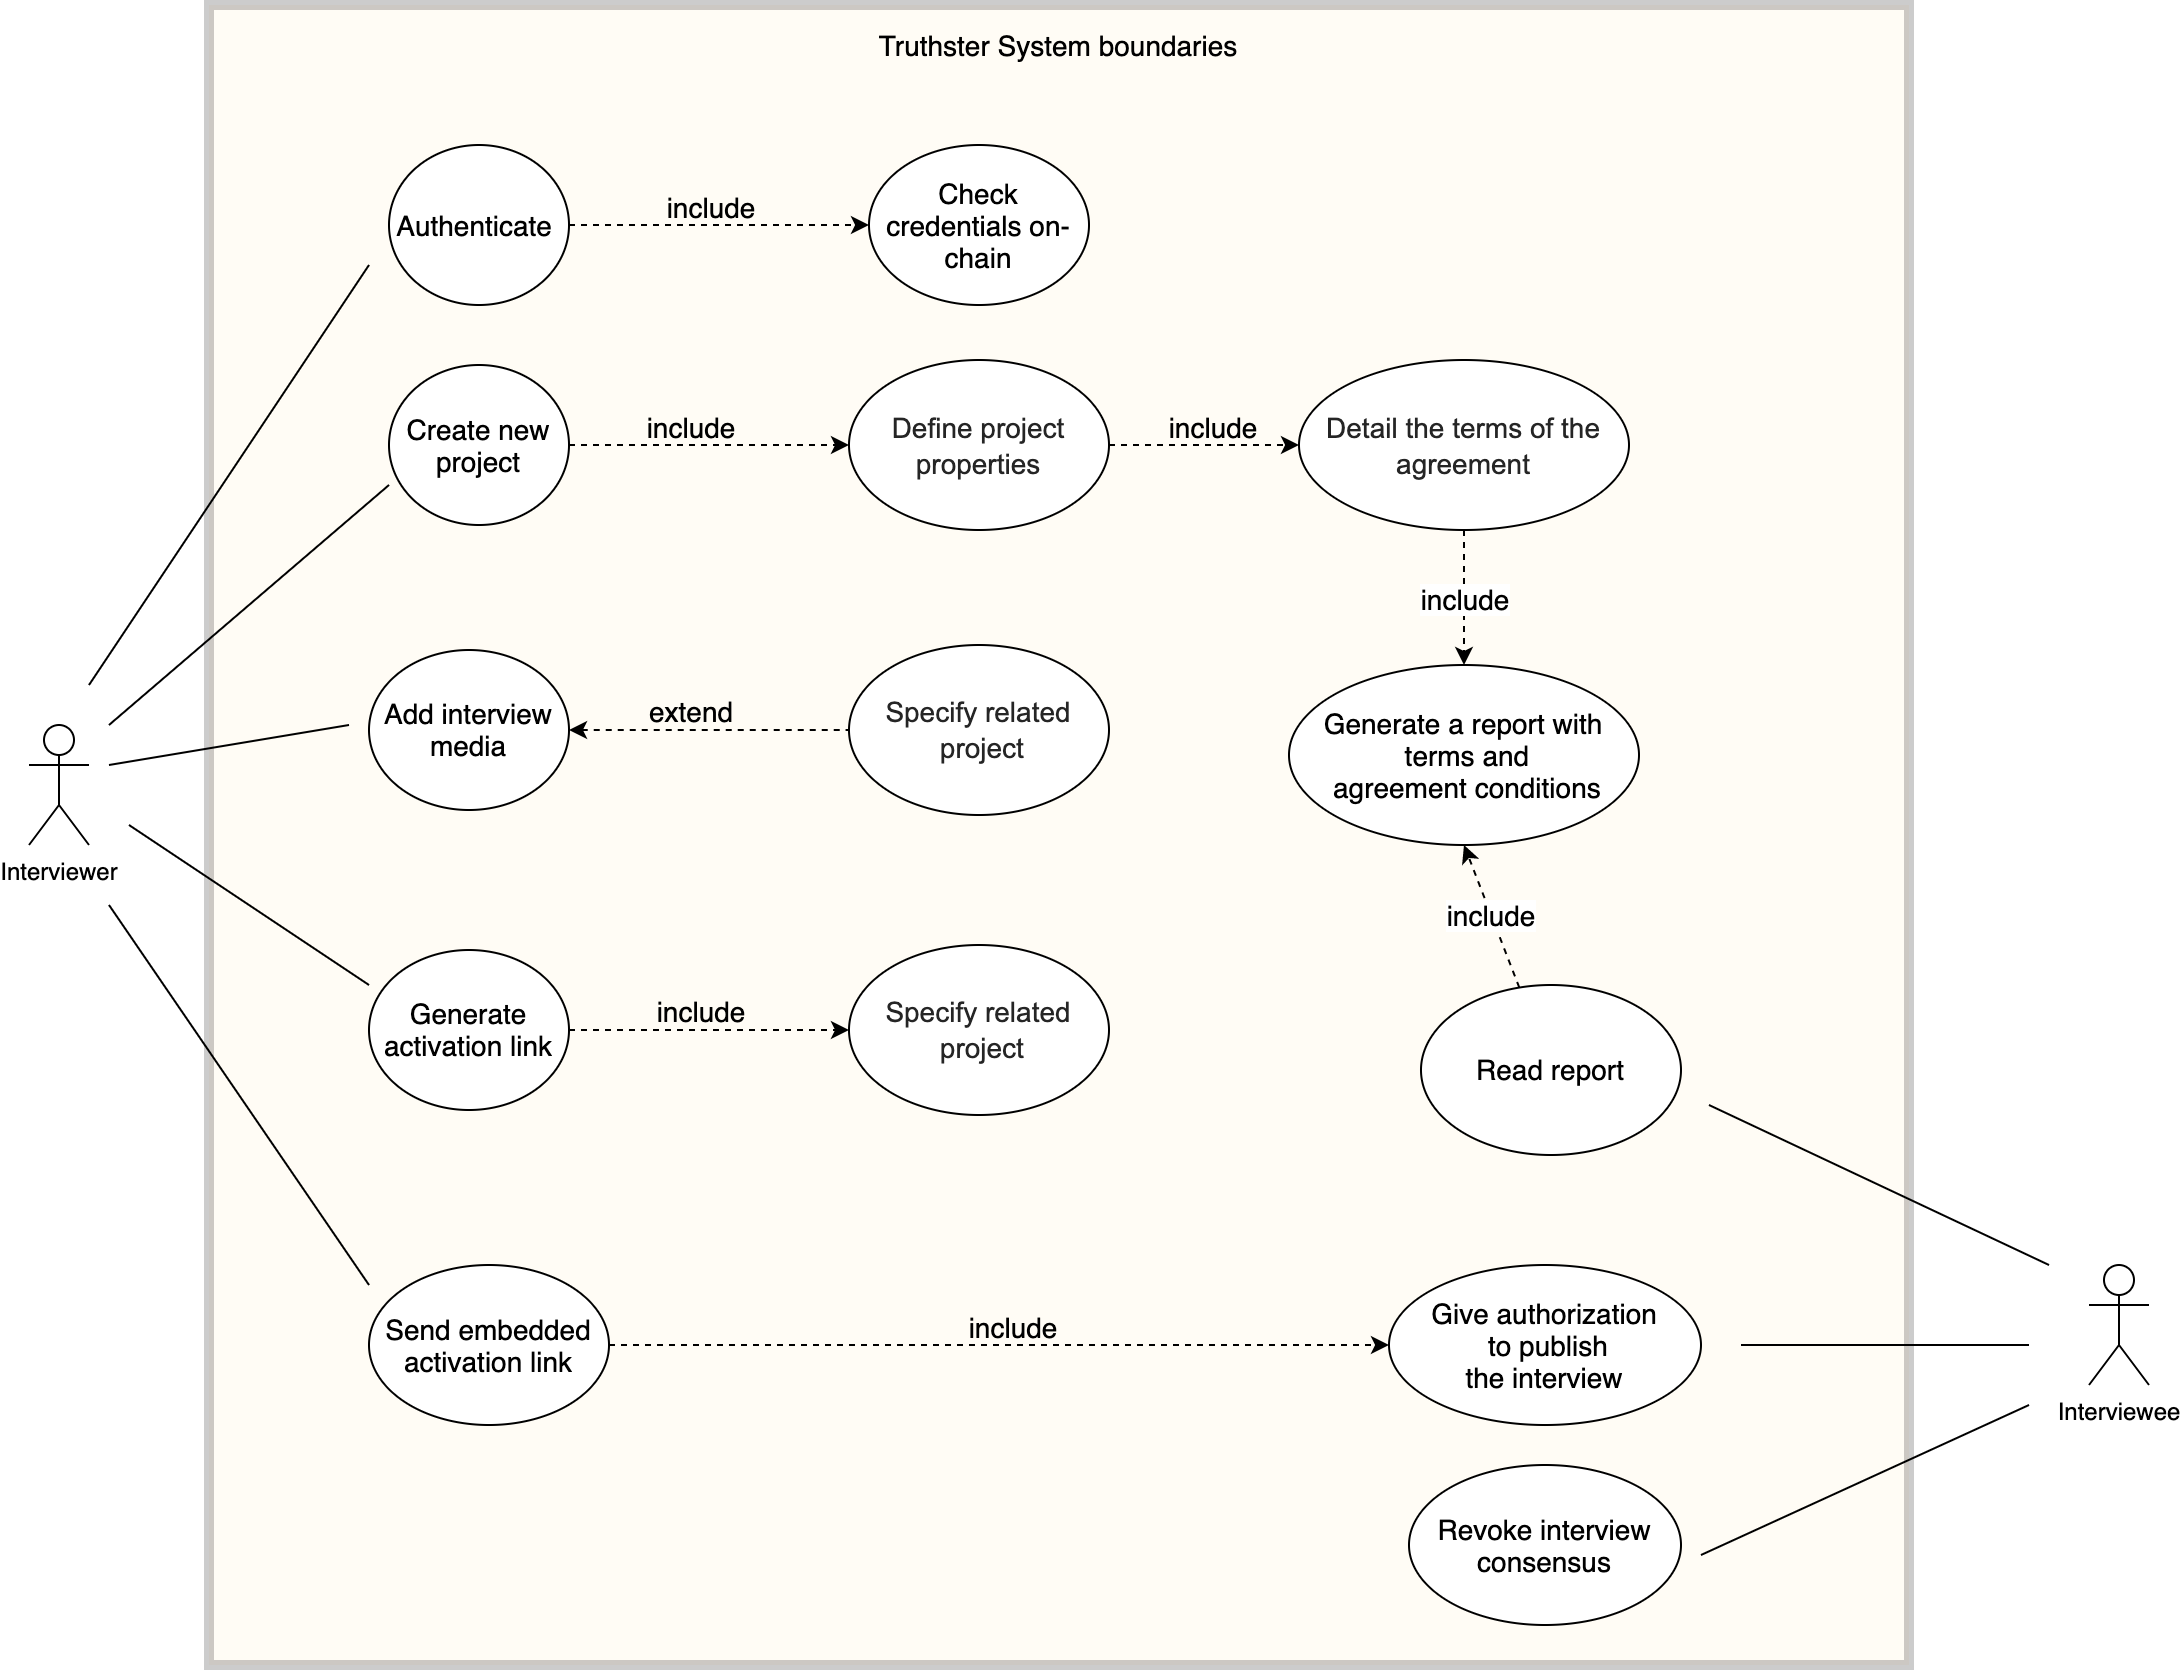
\includegraphics[width=0.8\textwidth]{images/truthster_use_cases.png}
    \caption{Truthster main use cases}
\end{figure}





\begin{itemize}

    \item Verifying the identity of an interviewer and the interviewee before and after the interview.
    \item Certifying the authenticity and integrity of the digital media (for example video interviews) through the use of blockchain technology (Alastria in our case).
    \item Embedding authorship and legal details (e.g., portrayal and data protection consent) into the digital media.
    \item Automating the generation of legal terms and conditions under which the content can circulate and can be used.
    \item Providing a tool for easy-to-use certification of media content, with emphasis on video interviews in our case.
    \item Achieving accountability in media creation by incorporating consent expressed by the interviewee and automating the generation of legal terms and conditions under which the content can circulate.
    \item Providing an easy-to-use tool for identity verification which can be useful for a wide range of other purposes (e.g., public authority identity check, restricted areas entering, consensus revoking)
    \item Providing a solution that is interoperable with other software and open (e.g., copyleft licenses) thus reducing lock-in effect for professionals who adopt it.
    
\end{itemize}

From these use cases we have derived some functional and non-functional requirements necessary to design the behavior and architecture of the Truthster system.\\

\section{Functional requirements}

The Truthster system has to be designed to provide a secure and efficient way for media creators to certify the validity of their digital media, specifically video interviews. In order to achieve this the system must meet a number of functional requirements to ensure that it is user-friendly, secure, and reliable. 
Below there is a list of functional requirements for our system:

\begin{itemize}

    \item The system must be able to generate a unique and tamper-proof hash of the interview video and metadata content:
    this hash value serves as a digital fingerprint of the interview, which can be used to verify the integrity of the original data. This is important for ensuring the authenticity and reliability of the interview, as it provides a secure way to prove that the content has not been altered in any way. By utilizing a blockchain like Alastria, the system can store this hash value in a decentralized and immutable manner, further increasing the security and trustworthiness of the interview content.
    \item The system must be able to store the hash, metadata and any other relevant information in a blockchain for secure, immutable record-keeping:
    this requirement ensures that all the information about the interview are stored in a blockchain, which is a decentralized and distributed ledger technology. This means that the information is not stored in a single location, but rather is spread across multiple nodes (called respectively Red-B and Red-T) in the network. This makes it extremely difficult for anyone to tamper with or alter the information because it would require changing the information on every node in the network. The blockchain in this way provides a secure and immutable record-keeping, meaning that once the information is recorded on the blockchain, it cannot be modified or deleted. Along with a database instance they provide a reliable and verifiable record of the interview that can be accessed at any time.
    \item The system must be able to send a link or QR code to the interviewee for them to review and agree to the GDPR compliant contract:
    this functional requirement ensures that the interviewee is provided with an easy and convenient way to review and agree to the GDPR compliant contract. This can be accomplished by sending a link or QR code to the interviewee via SMS or email. Once the link is opened or the QR code is scanned, the interviewee will be presented with the contract for review and agreement. This requirement is important to ensure that the interviewee is informed about their rights and responsibilities related to the interview and that their consent for the use of the interview material is obtained in a compliant and transparent manner. This is in line with the GDPR regulations, which require clear and informed consent for the processing of personal data.
    \item The system must be able to store the GPS position of the interviewee for added proof of location:
    the system must be able to collect and store the GPS position of the interviewee at the time of the interview for added proof of location. This information, along with the interview video and some metadata, will be stored in a MongoDB instance, providing an easily accessible record of the interview and its location. This feature adds an additional layer of security and validity to the interview, as it provides a physical reference point for the content, and allows for easy verification of the interview location. The use of MongoDB allows for a flexible schema approach, which is popular with development teams using agile methodologies.
    \item The system must be able to notify the interviewer when the process is complete:
    this requirement means that the system must be able to send a notification to the interviewer, through the mobile app or email, indicating that the process of uploading and storing the interview has been completed successfully. This will allow the interviewer to have real-time information about the status of the process and to access the stored interview data and metadata in the Alastria blockchain and MongoDB. This feature will also help to ensure that all steps of the process have been completed correctly and that the interviewer can proceed with the next step in the workflow.
    \item The system must have a history of all interviews stored in a separate database that can be accessed by the interviewer via REST API:
    this requirement means that the system must maintain a record of all interviews conducted using the Truthster app, including the relevant metadata, hash values, and other information. This history must be stored in a separate database, such as MongoDB, that can be accessed by the interviewer through a set of REST APIs. This allows the interviewer to easily view and manage their previous interviews, and provides them with a reliable and secure way to access the information stored in the database. The API's allows the interviewer to retrieve the data from the database in a structured manner, which can be used for reporting, analysis and other purposes. Additionally, the REST API's allow the interviewer to perform CRUD operations on the data, such as adding, updating and deleting. This ensures that the interviewer has full control over the data and can manage it effectively.
    \item The system must be able to automate the generation of legal terms and conditions for the use of the interview content:
    this requirement ensures that the legal terms and conditions for the use of the interview content are automatically generated based on predefined templates or rules. This includes terms related to data privacy and protection, as well as any other relevant legal agreements. This automation will save time and resources for the interviewer, while also ensuring that all legal requirements are met. Additionally, this will also provide a standardized process for the interviewee to review and agree to the legal terms before the interview content is shared. This will provide an added layer of protection for both parties involved.

\end{itemize}

\section{Non-functional requirements}

The Truthster system aims to provide a secure and efficient solution for the verification and certification of digital media. In order to achieve this goal, it must meet a number of non-functional requirements that ensure its reliability, scalability, and user-friendliness. The following is a list of non-functional requirements for the Truthster system:\\

\begin{itemize}

    \item Performance: The system must be able to handle a high volume of concurrent users and large amounts of data without experiencing significant lag or downtime.
    \item Usability: The system must be easy to use and understand for both interviewers and interviewees, with clear instructions and intuitive navigation.
    \item Security: The system must ensure the confidentiality and integrity of all data stored and transmitted, including personal data and media files.
    \item Scalability: The system must be able to handle an increasing amount of data and user without experiencing significant performance degradation.
    \item Compliance: The system must comply with relevant laws and regulations, including GDPR and copyright laws.
    \item Interoperability: The system must be able to integrate with other software and systems.

\end{itemize}

\chapter{Solution design}

Truthster is composed of a client-server architecture, with a front-end web/mobile application for interacting with the interviewer and interviewee, and a back-end that interacts with the front-end and services such as the Alastria Blockchain and storage service (mongoDB).\\
The process of using Truthster includes recording the audio/video material, logging into the mobile app, entering interview information and interviewee contact details, and choosing interview media. The app then authenticates the interviewer, calculates a hash of the media and uploads it to the storage server, sends a link to the interviewee, and stores the signed hash of the file in the blockchain via a smart contract on Alastria (AlastriaID library). After the previous steps are completed the interviewer is notified of the completion of the process, and can archive past interviews on their mobile app.\\
Basing our solution on the above description we can define the following components of the Truthster system:

\begin{enumerate}
    \item The front-end, which is a web/mobile application that interacts with the interviewer and interviewee. It uses REST APIs to exchange data with the back-end cloud.
    
    \item The back-end, which is a server that interacts with the front-end and with external services such as the Alastria blockchain and storage service.

    \item The Alastria Blockchain, which is a decentralized platform that provides proof of validity for the media files.

    \item The storage service, which stores the interview media files, metadata, and GPS positions of the interviewer and interviewee.
    
\end{enumerate}

\chapter{Implementation}

\chapter{Testing and validation}

\chapter{Conclusions}

%% Fine dei capitoli normali, inizio dei capitoli-appendice (opzionali)
\appendix

%\part{Appendici}

\chapter{Ganache}
Ganache is a personal blockchain for Ethereum development you can use to deploy contracts, develop your applications, and run tests. It is a tool that allows developers to create a virtual Ethereum blockchain on their local machine, which is useful for testing and developing smart contracts. Ganache creates a virtual blockchain that runs locally on your machine, which is separate from the live Ethereum network. This allows developers to test their contracts in a simulated environment, without the need for real Ether or the risk of interacting with the live network. Ganache also provides a user-friendly interface for interacting with the blockchain and managing accounts, making it easy for developers to test and debug their contracts.\\

Some possible disadvantages of using Ganache include:

\begin{enumerate}

    \item Limited scalability: Since Ganache is a personal blockchain running on a local machine, its scalability is limited by the resources of the machine it is running on. It may not be suitable for testing large-scale or high-traffic applications.
    \item Limited interoperability: Ganache is not connected to the live Ethereum network and therefore cannot interact with other networks or other instances of Ganache running on different machines. This can make it difficult to test and develop contracts that need to interact with other systems.
    \item Limited security: Ganache is intended for development and testing, and should not be used in production environments. It is not as secure as a live, public blockchain network and therefore may not be suitable for testing contracts that handle sensitive information or assets.
    \item Limited network effects: Ganache does not have the same network effects as the live Ethereum network, so it may not provide an accurate representation of how a contract will behave in a live environment.
    \item Limited real-world conditions: Ganache is a local blockchain, so it may not be able to simulate real-world conditions such as network delays, high load, and other environmental factors that can affect a contract's performance.

\end{enumerate}

It is worth noting that the above points are all related to the fact that Ganache is a personal blockchain that runs on a local machine, and it is not connected to the live Ethereum network. These limitations make it less suitable for testing and developing contracts that need to interact with other systems, handle sensitive information or assets, or be scalable and secure in a production environment.

    %% Parte conclusiva del documento; tipicamente per riassunto, bibliografia e/o indice analitico.
\backmatter

%% Riassunto (opzionale)
%\summary
%Maecenas tempor elit sed arcu commodo, dapibus sagittis leo egestas. Praesent at ultrices urna. Integer et nibh in augue mollis facilisis sit amet eget magna. Fusce at porttitor sapien. Phasellus imperdiet, felis et molestie vulputate, mauris sapien tincidunt justo, in lacinia velit nisi nec ipsum. Duis elementum pharetra lorem, ut pellentesque nulla congue et. Sed eu venenatis tellus, pharetra cursus felis. Sed et luctus nunc. Aenean commodo, neque a aliquam bibendum, mauris augue fringilla justo, et scelerisque odio mi sit amet diam. Nulla at placerat nibh, nec rutrum urna. Donec ut egestas magna. Aliquam erat volutpat. Phasellus vestibulum justo sed purus mattis, vitae lacinia magna viverra. Nulla rutrum diam dui, vel semper mi mattis ac. Vestibulum ante ipsum primis in faucibus orci luctus et ultrices posuere cubilia Curae; Donec id vestibulum lectus, eget tristique est.

%% Bibliografia (praticamente obbligatoria)
\bibliographystyle{plain_english}%% Carica l'omonimo file .bst, dove \languagename � la lingua attiva.
%% Nel caso in cui si usi un file .bib (consigliato)
\bibliography{thud}
%% Nel caso di bibliografia manuale, usare l'environment thebibliography.
\begin{thebibliography}{99}

    \bibitem{Why Proof-of-Work Is Not Viable in the Long-Term}
    Michael Zochowski, \href{https://medium.com/logos-network/why-proof-of-work-is-not-viable-in-the-long-term-dd96d2775e99}{Why Proof-of-Work Is Not Viable in the Long-Term}

    \bibitem{VergeAttack}
    CCN, \href{https://www.ccn.com/privacy-coin-verge-succumbs-to-51-attack-again/}{Privacy Coin Verge Succumbs to 51\% Attack [Again]}

    \bibitem{factmata}
    Factmata, \href{https://factmata.com/}{Factmata}

    \bibitem{NewsWhip}
    NewsWhip, \href{https://www.newswhip.com/}{NewsWhip}

    \bibitem{veracity.ai}
    Veracity.AI, \href{https://veracityai.com/en/}{veracity.ai}

    \bibitem{Factcheck}
    Factcheck.org, \href{https://www.factcheck.org/}{FactCheck.org}

    \bibitem{mediabiasfactcheck}
    Media Bias / Fact Check, \href{https://mediabiasfactcheck.com/}{Media Bias / Fact Check}

    \bibitem{googleVerificationToolkit}
    Google News Lab Verification Toolkit, \href{https://newsinitiative.withgoogle.com/resources/journalism/}{Journalism Resources}

    \bibitem{EXP51Attack}
    Expanse was 51\% attacked, \href{https://gist.github.com/metalicjames/01222049f95f85df8c0eb253de54848b}{Expanse (EXP) was 51\% attacked}

    \bibitem{BTCG51Attack}
    Bitcoin Gold 51\% attack, \href{https://gist.github.com/metalicjames/71321570a105940529e709651d0a9765}{Bitcoin Gold (BTG) was 51\% attacked}

    \bibitem{VTC51Attack}
    Vertcoin was 51\% attacked, \href{https://gist.github.com/metalicjames/f2acdb9ef448ec5298173b36c7c54133}{Vertcoin (VTC) was 51\% attacked}

    \bibitem{LCC51Attack}
    Litecoin Cash was 51\% attacked, \href{https://gist.github.com/metalicjames/82a49f8afa87334f929881e55ad4ffd7}{Litecoin Cash (LCC) was 51\% attacked}

    \bibitem{SelfishMiningDefinition}
    Investopedia, \href{https://www.investopedia.com/terms/s/selfish-mining.asp}{Selfish Mining Definition}

    \bibitem{NothingAtStake}
    Medium, \href{https://medium.com/coinmonks/understanding-proof-of-stake-the-nothing-at-stake-theory-1f0d71bc027}{Understanding Proof of Stake: The Nothing at Stake Theory}

    \bibitem{LongRangeAttack}
    Medium, \href{https://blog.positive.com/rewriting-history-a-brief-introduction-to-long-range-attacks-54e473acdba9}{Rewriting History: A Brief Introduction to Long Range Attacks}


    \bibitem{}
    , \href{}{}

\end{thebibliography}

%% Per l'indice analitico, usare il pacchetto makeidx (o analogo).

\end{document}

--- Istruzioni per l'aggiunta di nuove lingue ---
Per ogni nuova lingua utilizzata aggiungere nel preambolo il seguente spezzone:
    \addto\captionsitalian{%
        \def\abstractname{Sommario}%
        \def\acknowledgementsname{Ringraziamenti}%
        \def\authorcontactsname{Contatti dell'autore}%
        \def\candidatename{Candidato}%
        \def\chairname{Direttore}%
        \def\conclusionsname{Conclusioni}%
        \def\cosupervisorname{Co-relatore}%
        \def\cosupervisorsname{Co-relatori}%
        \def\cyclename{Ciclo}%
        \def\datename{Anno accademico}%
        \def\indexname{Indice analitico}%
        \def\institutecontactsname{Contatti dell'Istituto}%
        \def\introductionname{Introduzione}%
        \def\prefacename{Prefazione}%
        \def\reviewername{Controrelatore}%
        \def\reviewersname{Controrelatori}%
        %% Anno accademico
        \def\shortdatename{A.A.}%
        \def\summaryname{Riassunto}%
        \def\supervisorname{Relatore}%
        \def\supervisorsname{Relatori}%
        \def\thesisname{Tesi di \expandafter\ifcase\csname thud@target\endcsname Laurea\or Laurea Magistrale\or Dottorato\fi}%
        \def\tutorname{Tutor aziendale%
        \def\tutorsname{Tutor aziendali}%
    }
sostituendo a "italian" (nella 1a riga) il nome della lingua e traducendo le varie voci.
